%%%%%%%%%%%%%%%%%%%% author.tex %%%%%%%%%%%%%%%%%%%%%%%%%%%%%%%%%%%
%
% sample root file for your "contribution" to a contributed volume
%
% Use this file as a template for your own input.
%
%%%%%%%%%%%%%%%% Springer %%%%%%%%%%%%%%%%%%%%%%%%%%%%%%%%%%


% RECOMMENDED %%%%%%%%%%%%%%%%%%%%%%%%%%%%%%%%%%%%%%%%%%%%%%%%%%%
\documentclass[graybox]{svmult}

% choose options for [] as required from the list
% in the Reference Guide

\usepackage{type1cm}        % activate if the above 3 fonts are
                            % not available on your system
%
\usepackage{makeidx}         % allows index generation
\usepackage{graphicx}        % standard LaTeX graphics tool
                             % when including figure files
\usepackage{multicol}        % used for the two-column index
\usepackage[bottom]{footmisc}% places footnotes at page bottom


\usepackage{newtxtext}       % 
\usepackage{newtxmath}       % selects Times Roman as basic font

\usepackage{booktabs}       % Booktabs Table Style

\usepackage{graphicx}       % To frame graphic images
\usepackage[export]{adjustbox}

\usepackage[section]{placeins} % Forces an image to be displayed in it's section
%\usepackage{draftwatermark}



% see the list of further useful packages
% in the Reference Guide

\makeindex             % used for the subject index
                       % please use the style svind.ist with
                       % your makeindex program

%%%%%%%%%%%%%%%%%%%%%%%%%%%%%%%%%%%%%%%%%%%%%%%%%%%%%%%%%%%%%%%%%%%%%%%%%%%%%%%%%%%%%%%%%

\DeclareUnicodeCharacter{2212}{-}
\DeclareUnicodeCharacter{22C5}{-}

\begin{document}

%\SetWatermarkText{DRAFT}
%\SetWatermarkScale{1}


\title*{A new breeding crossover approach for evolutionary algorithms}
%


\titlerunning{A new breeding crossover approach for evolutionary algorithms}
% Use \titlerunning{Short Title} for an abbreviated version of
% your contribution title if the original one is too long
\author{J. C. Felix-Saul, Mario García-Valdez}
% Use \authorrunning{Short Title} for an abbreviated version of
% your contribution title if the original one is too long
\institute{J. C. Felix-Saul \at TecNM, Tijuana Institute of Technology, Tijuana, Mexico, \email{jose.felix201@tectijuana.edu.mx}
\and Mario García-Valdez \at TecNM, Tijuana Institute of Technology, Tijuana, Mexico, \email{mario@tectijuana.edu.mx}}
%
% Use the package "url.sty" to avoid
% problems with special characters
% used in your e-mail or web address
%
\maketitle

\abstract*{In a previous work, we introduced a population-based, bio-inspired algorithm. The proposed algorithm is inspired by the biological animal life cycle, consisting of the birth, growth, reproduction, and death stages. Our algorithm was initially based on the canonical Genetic Algorithm (GA), where all the individuals have a genotype (chromosome). One difference to highlight in our algorithm is that both the crossing and the mutation are executed through independent processes that randomly affect the population. This paper focuses on breeding, whereas in earlier versions of the algorithm, we used the traditional GA one-point crossover. In this paper, we propose a different alternative to the classical approach, where part of the genetic information is directly copied to each of the offspring in the crossover operator, where this type of crossover may not perform well in continuous optimization problems. In this proposal, we use the parent's genetic information for each gene, using those values as lower and upper bounds of a range, where a random value within that range determines the new value for that gene index of the offspring. This is similar to what is used by algorithms such as Differential Evolution, where we consider our proposal as a variation of existing proposals. We expect this new operator to allow the offspring to continue exploring new search spaces with the birth of individuals. This paper uses the benchmark functions introduced in the Competition on Evolutionary Computation for the 2017 edition (CEC2017) to compare the traditional one-point crossover and our proposed strategy. Experimental results indicate that our proposed operator may be a good alternative for the canonical crossover.}



\abstract{In a previous work, we introduced a population-based, bio-inspired algorithm. The proposed algorithm is inspired by the biological animal life cycle, consisting of the birth, growth, reproduction, and death stages. Our algorithm was initially based on the canonical Genetic Algorithm (GA), where all the individuals have a genotype (chromosome). One difference to highlight in our algorithm is that both the crossing and the mutation are executed through independent processes that randomly affect the population. This paper focuses on breeding, whereas in earlier versions of the algorithm, we used the traditional GA one-point crossover. In this paper, we propose a different alternative to the classical approach, where part of the genetic information is directly copied to each of the offspring in the crossover operator, where this type of crossover may not perform well in continuous optimization problems. In this proposal, we use the parent's genetic information for each gene, using those values as lower and upper bounds of a range, where a random value within that range determines the new value for that gene index of the offspring. This is similar to what is used by algorithms such as Differential Evolution, where we consider our proposal as a variation of existing proposals. We expect this new operator to allow the offspring to continue exploring new search spaces with the birth of individuals. In this paper, we use the benchmark functions introduced in the Competition on Evolutionary Computation for the 2017 edition (CEC2017) to compare the traditional one-point crossover and our proposed strategy. Experimental results indicate that our proposed operator may be a good alternative for the canonical crossover.}

%\keywords{Distributed Bioinspired Algorithms \and Genetic Algorithms \and Cloud Computing.}

\newpage
\section{Introduction}
    \label{sec:1}

    Biologically inspired algorithms are a very effective technique to solve complex optimization problems\cite{castillo2019comparative,valdez2021swarm,acherjee2020ultrasonic}. Traditionally, nature-inspired algorithms are developed with a sequential perspective\cite{porto2018evolutionary,back1996evolutionary}, meaning that all tasks execute one step at a time, where all processes must wait until the current task finishes before proceeding (synchronous perspective). One solution to this issue is working with cloud computing\cite{valdez2021container,garcia2015evospace,merelo2016nodio} and using distributed architectures. 

    In previous work, we introduced a population-based, bio-inspired algorithm\cite{Felix-Saul2022,Felix-Saul2023}. The proposed algorithm is inspired by the biological animal life cycle, consisting of the birth, growth, reproduction, and death stages\cite{read1968system}. Our algorithm was initially based on the canonical Genetic Algorithm (GA)\cite{holland1992genetic,holland1984genetic}, where all the individuals have a genotype (chromosome) constructed by a list of values, where we compute the individual's fitness using an evaluation function that represents the problem we wish to solve.
    
    The algorithm's main objective is to abstract how the animal life cycle performs in nature, where at any given time, newborn individuals are integrated into the population and partake in communal evolution. Progressively, all individuals grow and mature, consequently suffering changes that we represent with mutations in our design. In our modeling, we enforced the survival of the fittest. As in nature, death randomly tests every living organism to help maintain balance in the numbers in the population; therefore, it is independent of the individual's age. However, fitness will be the main factor in prolonging its longevity.

    One essential feature to highlight in the algorithm is that it doesn't use the concept of generations in the evolution. Our strategy views the population as a set of candidate solutions that evolve continuously over time, which allows individuals of multiple ages to reproduce and generate new offspring, reflecting nature's actual behavior. Another difference to highlight in our algorithm is that both reproduction (crossover) and growth (mutation) execute through independent processes that randomly affect the population. Figure~\ref{fig.algorithm_model} displays the general model concept for the Animal Life Cycle Algorithm (ALCA).

    We propose a new reproduction alternative in this research: a new breeding crossover approach for evolutionary algorithms using the classic one-point crossover as a reference to our proposal. We performed comparison experiments using the mathematical benchmark functions introduced in the Competition on Evolutionary Computation for the 2017 edition (CEC-2017) for evaluation. We finalize with a statistical Z-Test with a ninety-five percent confidence level to determine the best alternative.

    One of the most important contributions of this research is that it proposes a new crossing alternative for the reproduction of individuals in a population. This strategy is practical in evolutionary algorithms where the individual's information has a structure similar to the genetic code's. With some tinkering, this strategy could be valuable in other algorithms\cite{venter2003particle,wang2018particle}, such as Particle Swarm Optimization (PSO).

    We organized this paper in the following structure. First, we illustrate our alternative crossover proposal, from the inspiration to a detailed example. The proposal section~\ref{section.proposal} compares the canonical one-point crossover with our crossover solution. We continue with the experiments section~\ref{section.experiments} with our experiment configuration and results. We include the analysis and description of some of our research discoveries in the discussion section~\ref{section.discussion}. The conclusions section~\ref{section.conclusions} finalizes presenting some deductions founded on the study of our experiments.


    \begin{figure}[!ht]
        \centering
        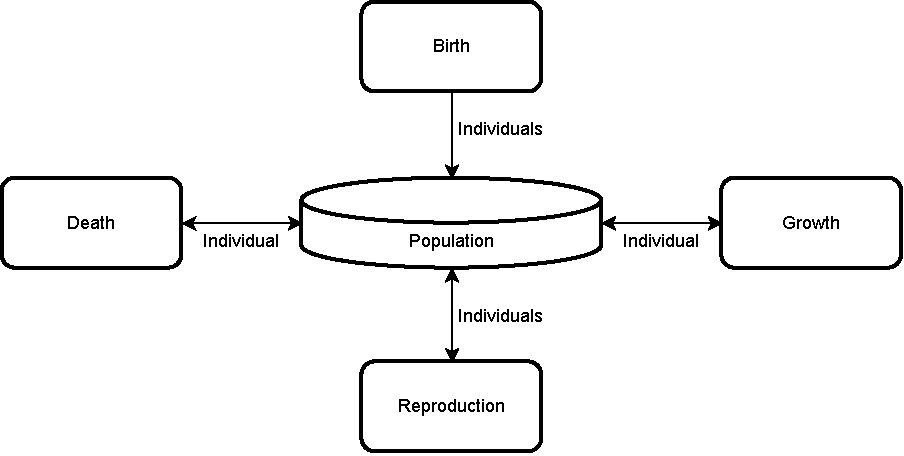
\includegraphics[width=0.90\linewidth]{img/fig_algorithm_model.pdf}
        \caption{Animal Life Cycle Algorithm model.} \label{fig.algorithm_model}
        \end{figure}


\section{Proposal}
    \label{section.proposal}

    Let's imagine that the colors black and white fell in love and had children. If we had to guess what color their offspring would be, it could only be predictable its children's color would be inside the domain shown in Figure~\ref{fig.grayscale_continuous}.

    \begin{figure}[!ht]
        \centering
        
\includegraphics[width=0.70\linewidth]{img/fig_grayscale_continuous.pdf}
        \caption{Black and white offspring, predictable color domain.} \label{fig.grayscale_continuous}
        \end{figure}

    If we replace the colors black and white with values 0 and 1, respectively, how many values can we find in between? We could replace attributes, switching from color to height, strength, agility, or any other feature we might need to focus on. The parents' attribute values will determine how their offspring's attributes are defined. This paper focuses on breeding (or reproduction), whereas in earlier versions of the algorithm, we used the traditional (GA) one-point crossover. 

    \subsection{Crossover Proposal}

    In this document, we propose a different technique to the canonical approach One Point Crossover, where part of the genetic information is copied directly to each offspring in the crossover operator. This type of crossover may fail to perform successfully in continuous optimization problems. Figure~\ref{fig.onepoint_crossover} provides an example of the One Point Crossover.

    \begin{figure}[!ht]
        \centering
        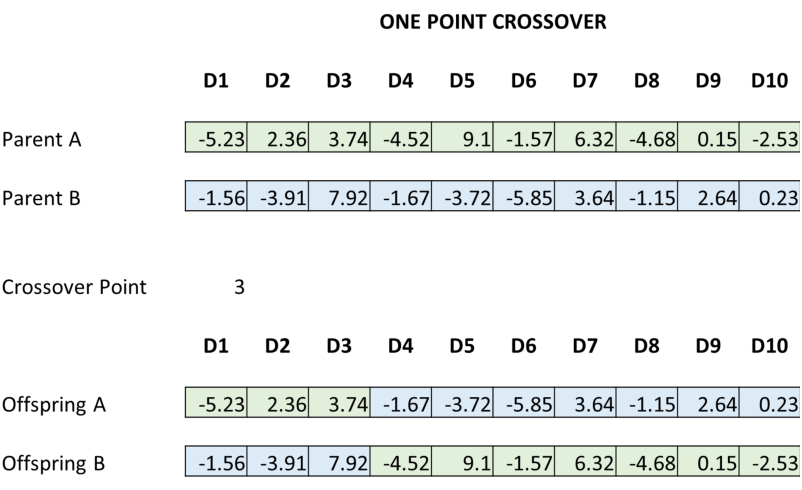
\includegraphics[width=0.50\linewidth]{img/fig_onepoint_crossover.pdf}
        \caption{Classical approach example for the One Point Crossover, with crossover point 3.} \label{fig.onepoint_crossover}
        \end{figure}

    In this proposal, we use the parent's genetic information for each gene, using those values as lower and upper bounds of a range, where a random value within that range determines the new value for that gene index of the offspring. Our proposal example for the Continuous Range Crossover is displayed in Figure~\ref{fig.contrange_crossover}, where it should be noted that we construct a template that will be used for all the offspring generated by each couple.

    \begin{figure}[!ht]
        \centering
        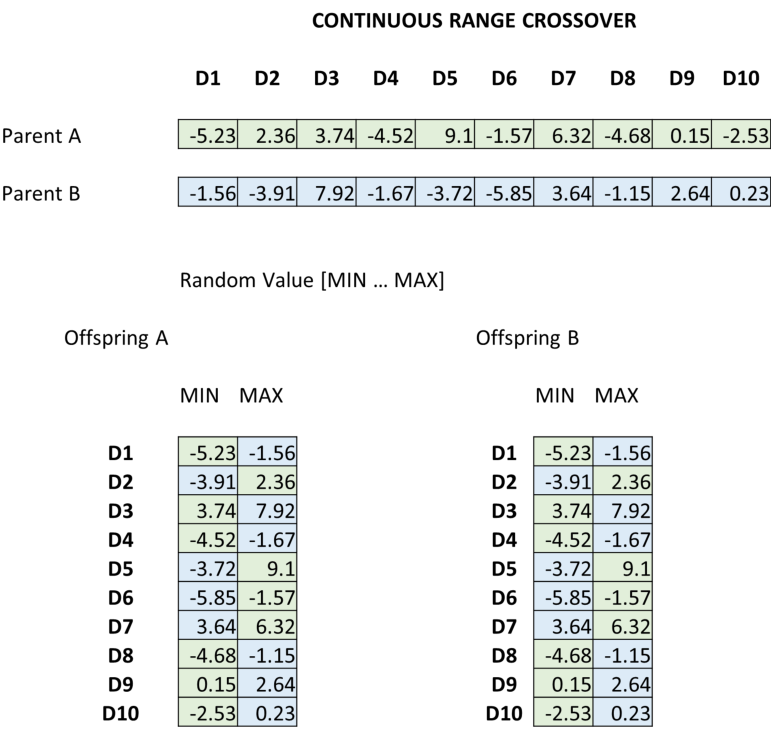
\includegraphics[width=0.50\linewidth]{img/fig_contrange_crossover.pdf}
        \caption{Our proposal example for the Continuous Range Crossover mating the same couple of individuals.} \label{fig.contrange_crossover}
        \end{figure}        
    
    \FloatBarrier


\section{Experiments}
    \label{section.experiments}

    To validate our proposal, we performed experiments using the mathematical benchmark functions introduced in the Competition on Evolutionary Computation for the 2017 edition (CEC-2017) for evaluation to compare the traditional one-point crossover and our proposed strategy. We finalize with a statistical Z-Test with a ninety-five percent confidence level to determine the best alternative. Table~\ref{tab.benchmark_functions} lists the thirty mathematical benchmark functions used for evaluation, to obtain the comparison results shown in our research.

    \begin{table}[]
    \scriptsize
    \centering
    \caption{Mathematical benchmark functions introduced in the Competition on Evolutionary Computation for the 2017 edition (CEC-2017).}\label{tab.benchmark_functions}    
    \begin{tabular}{@{}cllcl@{}}
    \toprule
    \multicolumn{5}{c}{\textbf{CEC-2017 Mathematical Benchmark Functions}} \\ \midrule
    \textbf{Fx} & \textbf{Function Name} &  & \textbf{Fx} & \textbf{Function Name} \\
    F1 & Shifted and Rotated   Bent Cigar Function &  & F16 & Hybrid function 6 \\
    F2 & Shifted and Rotated   Sum of Different Power Function &  & F17 & Hybrid function 7 \\
    F3 & Shifted and Rotated   Zakharov Function &  & F18 & Hybrid function 8 \\
    F4 & Shifted and Rotated   Rosenbrock's Function &  & F19 & Hybrid function 9 \\
    F5 & Shifted and Rotated   Rastrigin's Function &  & F20 & Hybrid function 10 \\
    F6 & Shifted and Rotated   Schaffer F7 Function &  & F21 & Composition function   1 \\
    F7 & Shifted and Rotated   Lunacek Bi-Rastrigin's Function &  & F22 & Composition function   2 \\
    F8 & Shifted and Rotated   Non-Continuous Rastrigin's Function &  & F23 & Composition function   3 \\
    F9 & Shifted and Rotated   Levy Function &  & F24 & Composition function   4 \\
    F10 & Shifted and Rotated   Schwefel's Function &  & F25 & Composition function   5 \\
    F11 & Hybrid function 1 &  & F26 & Composition function   6 \\
    F12 & Hybrid function 2 &  & F27 & Composition function   7 \\
    F13 & Hybrid function 3 &  & F28 & Composition function   8 \\
    F14 & Hybrid function 4 &  & F29 & Composition function   9 \\
    F15 & Hybrid function 5 &  & F30 & Composition function   10 \\ \bottomrule
    \end{tabular}
    \end{table}


    \subsection{Experimental Configuration}

    We used the Animal Life Cycle Algorithm (ALCA) for our experiments, switching between the breeding strategies (One Point and Continuous Range Crossover) with the same general setup. Table~\ref{tab.general_configuration} displays the General Configuration used to run the experiments for our research, where all the values remained consistent during all the stages of the test runs.

    For each of the thirty mathematical benchmark functions from the CEC-2017, we evaluated the ten and thirty dimensions, where we performed fifty-one runs per dimension. To find and determine the best alternative finalized with a statistical Z-Test with a ninety-five percent confidence level.

    \begin{table}[]
    \scriptsize
    \centering
    \caption{Animal Life Cycle Algorithm (ALCA) General Configuration.}\label{tab.general_configuration}    
    \begin{tabular}{@{}ll@{}}
    \toprule
    \multicolumn{2}{l}{\textbf{ALCA   General Configuration}} \\ \midrule
    \textbf{Function name} & \textbf{ALL} \\
    Population & 500 \\
    Evaluations & 10,000 * Dim \\
    Crossover rate & 100 \\
    Mutation rate & 7 \\
    Max age & 5 \\
    Tournament rep. & 100 \\
    Sample size & 20 \\
    Base approval & 80 \\
    Goal approval & 200 \\ \bottomrule
    \end{tabular}
    \end{table}

    \FloatBarrier


    \subsection{Experimental Results}

    We describe how to interpret the results presented in our Box and Whisker charts for each mathematical function. We display the ten and thirty-dimension charts on the left and right sides. We can find the results accumulated in 51 runs, in green color the One Point crossover, and in blue color the Continuous Range crossover. The closer the error results get to the zero value, the better.

    \begin{figure}[!ht]
        \begin{minipage}[h]{0.49\linewidth}
            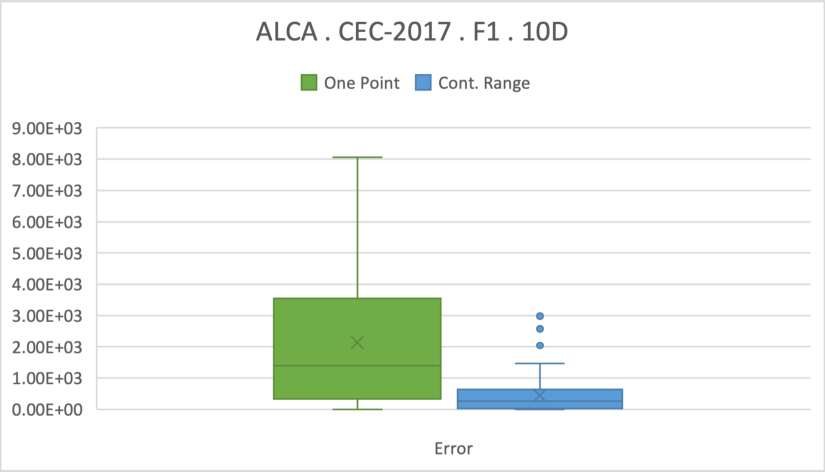
\includegraphics[width=1\linewidth]{img/fig_experiment_F1x10D.pdf} 
        \end{minipage}
        \hfill
        \vspace{0.05 cm}
        \begin{minipage}[h]{0.49\linewidth}
            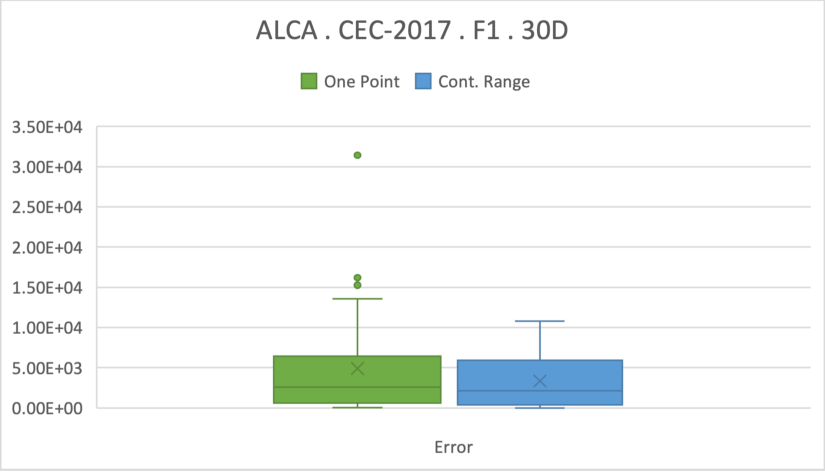
\includegraphics[width=1\linewidth]{img/fig_experiment_F1x30D.pdf} 
        \end{minipage}
        \vfill
        \vspace{0.05 cm}
        \begin{minipage}[h]{0.49\linewidth}
            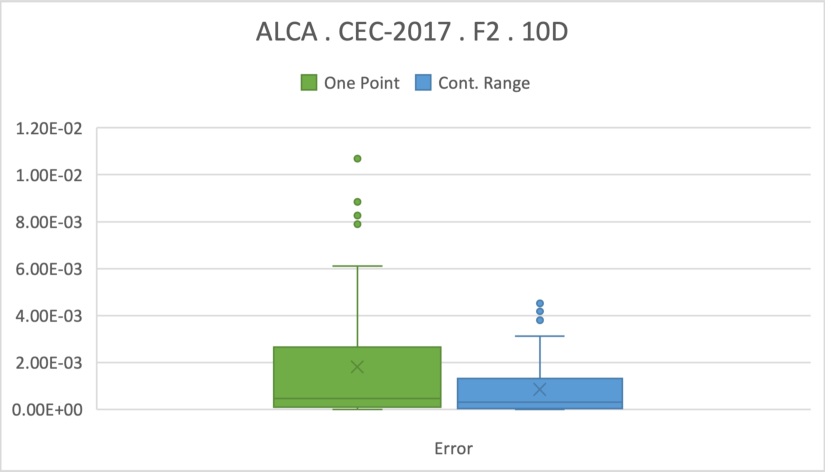
\includegraphics[width=1\linewidth]{img/fig_experiment_F2x10D.pdf} 
        \end{minipage}
        \hfill
        \begin{minipage}[h]{0.49\linewidth}
            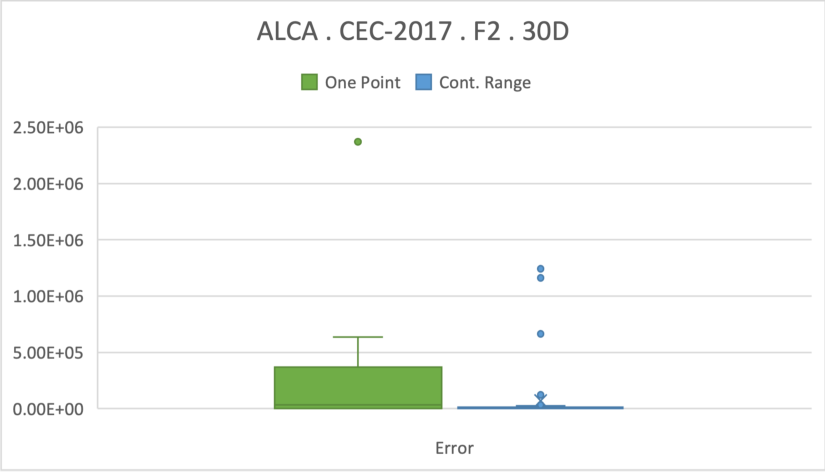
\includegraphics[width=1\linewidth]{img/fig_experiment_F2x30D.pdf} 
        \end{minipage}
        
        \caption{Box and Whisker charts for mathematical functions F1 and F2. We display the ten and thirty-dimension charts on the left and right sides for the results accumulated in 51 runs.} \label{fig.experiment_F1-F2}
    \end{figure}

    \FloatBarrier

    \begin{figure}[!ht]
        \begin{minipage}[h]{0.49\linewidth}
            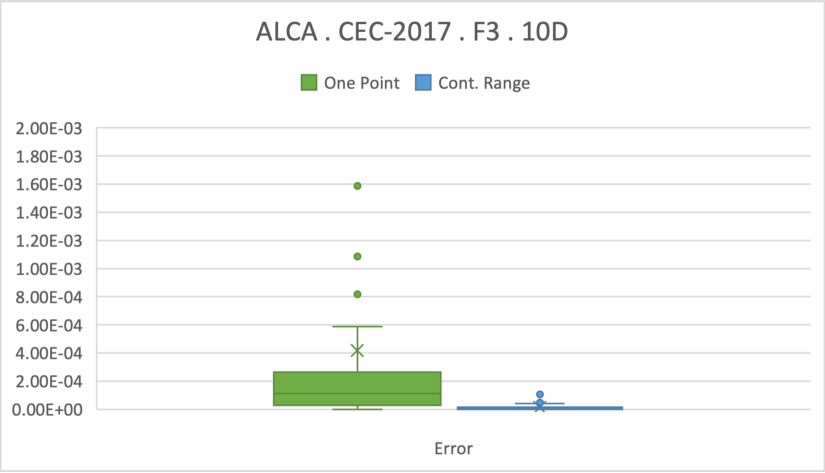
\includegraphics[width=1\linewidth]{img/fig_experiment_F3x10D.pdf} 
        \end{minipage}
        \hfill
        \vspace{0.05 cm}
        \begin{minipage}[h]{0.49\linewidth}
            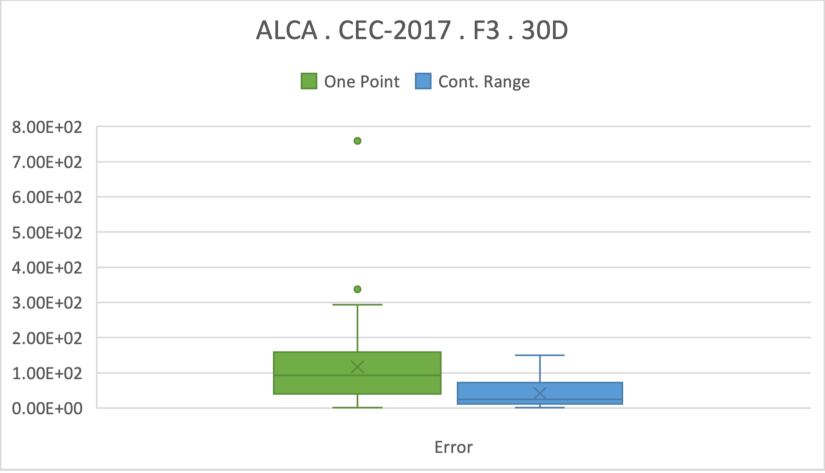
\includegraphics[width=1\linewidth]{img/fig_experiment_F3x30D.pdf} 
        \end{minipage}
        \vfill
        \vspace{0.05 cm}
        \begin{minipage}[h]{0.49\linewidth}
            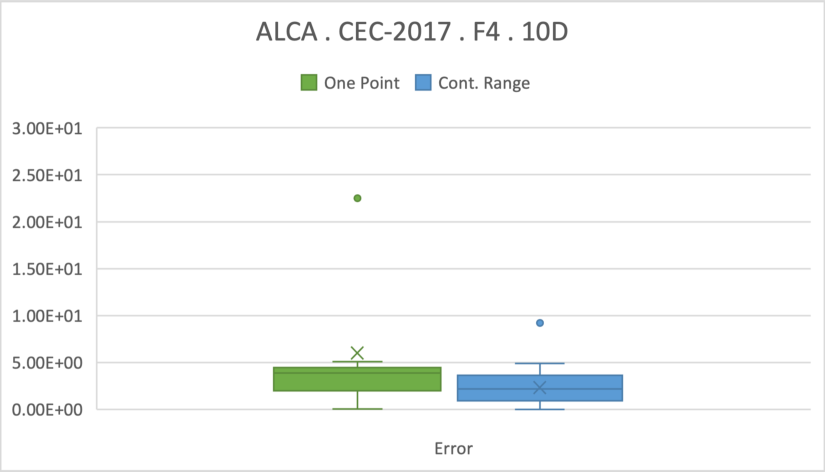
\includegraphics[width=1\linewidth]{img/fig_experiment_F4x10D.pdf} 
        \end{minipage}
        \hfill
        \begin{minipage}[h]{0.49\linewidth}
            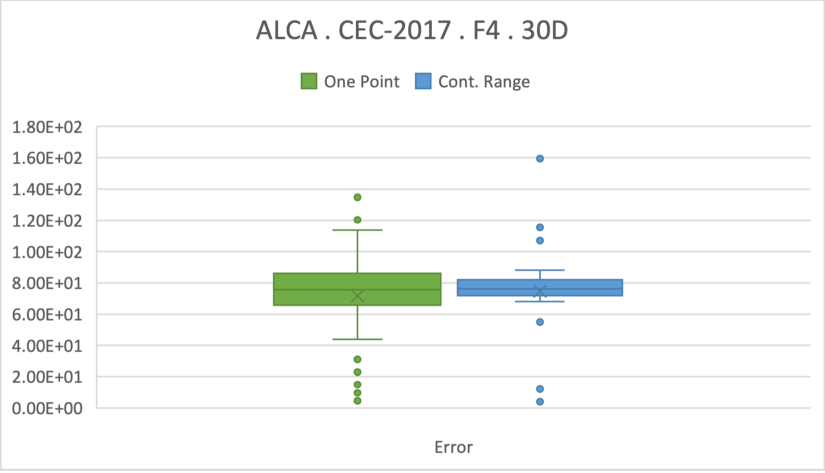
\includegraphics[width=1\linewidth]{img/fig_experiment_F4x30D.pdf} 
        \end{minipage}
        \vfill
        \vspace{0.05 cm}
        \begin{minipage}[h]{0.49\linewidth}
            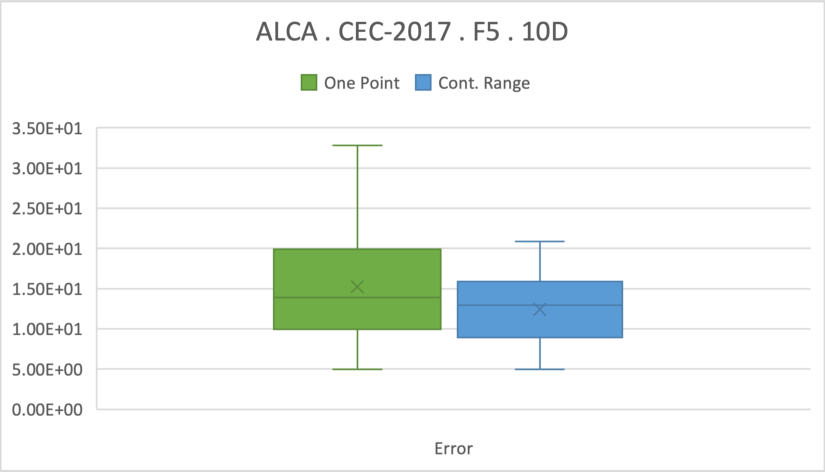
\includegraphics[width=1\linewidth]{img/fig_experiment_F5x10D.pdf} 
        \end{minipage}
        \hfill
        \begin{minipage}[h]{0.49\linewidth}
            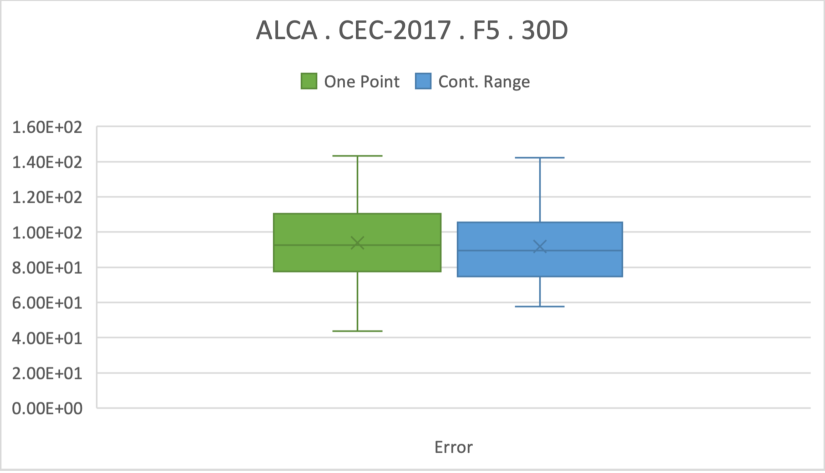
\includegraphics[width=1\linewidth]{img/fig_experiment_F5x30D.pdf} 
        \end{minipage}
        \vfill
        \vspace{0.05 cm}
        \begin{minipage}[h]{0.49\linewidth}
            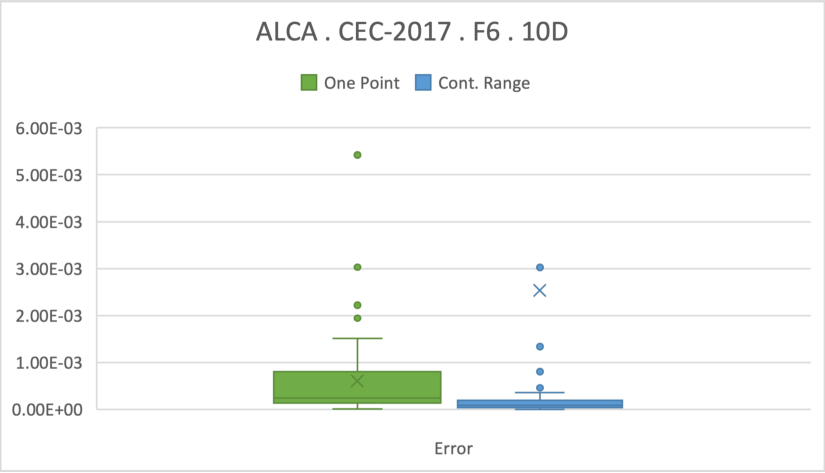
\includegraphics[width=1\linewidth]{img/fig_experiment_F6x10D.pdf} 
        \end{minipage}
        \hfill
        \begin{minipage}[h]{0.49\linewidth}
            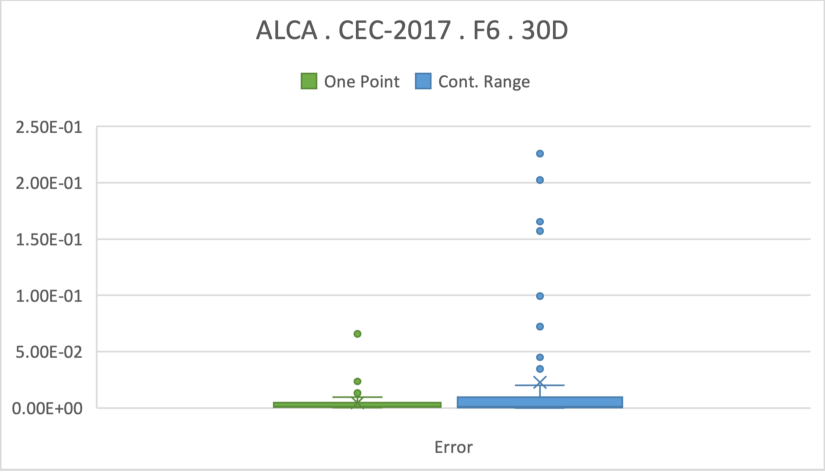
\includegraphics[width=1\linewidth]{img/fig_experiment_F6x30D.pdf} 
        \end{minipage}
        \vfill
        \vspace{0.05 cm}
        \begin{minipage}[h]{0.49\linewidth}
            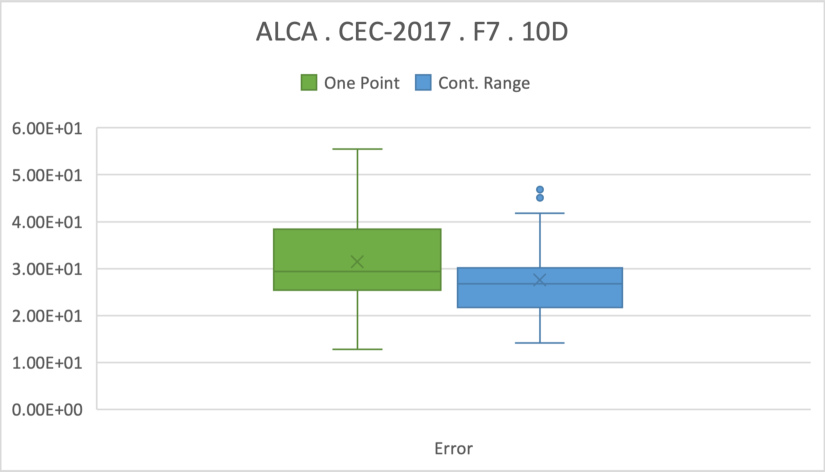
\includegraphics[width=1\linewidth]{img/fig_experiment_F7x10D.pdf} 
        \end{minipage}
        \hfill
        \begin{minipage}[h]{0.49\linewidth}
            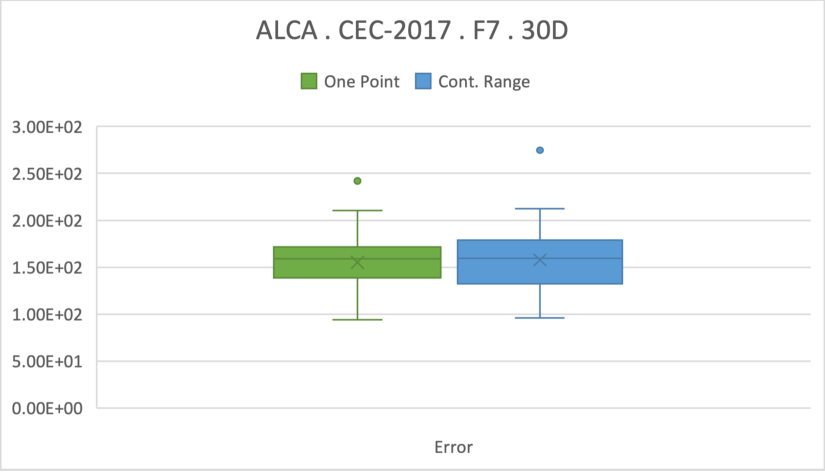
\includegraphics[width=1\linewidth]{img/fig_experiment_F7x30D.pdf} 
        \end{minipage}
        \vfill
        \vspace{0.05 cm}
        \begin{minipage}[h]{0.49\linewidth}
            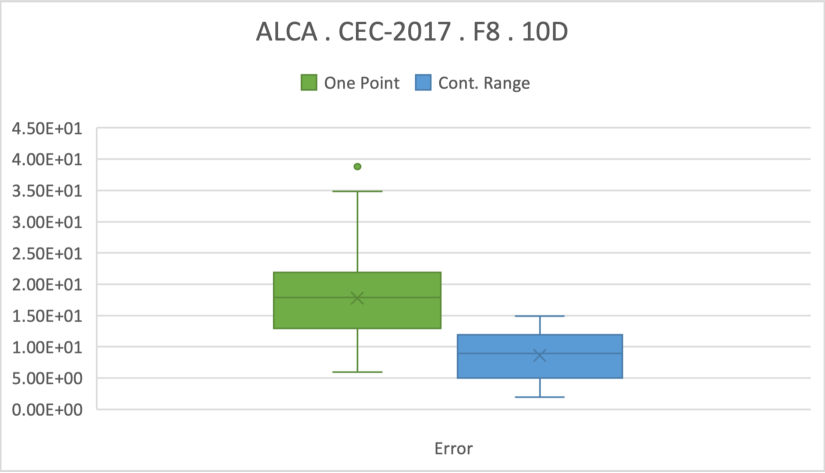
\includegraphics[width=1\linewidth]{img/fig_experiment_F8x10D.pdf} 
        \end{minipage}
        \hfill
        \begin{minipage}[h]{0.49\linewidth}
            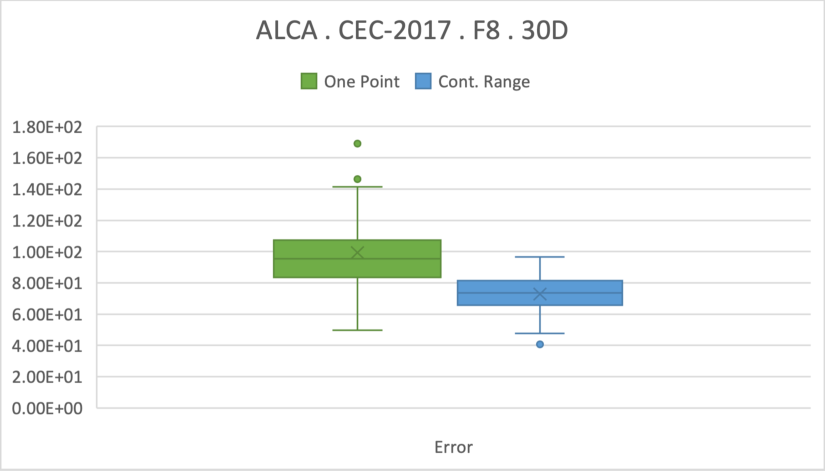
\includegraphics[width=1\linewidth]{img/fig_experiment_F8x30D.pdf} 
        \end{minipage}

        \caption{Box and Whisker charts for mathematical functions F3 to F8. We display the ten and thirty-dimension charts on the left and right sides for the results accumulated in 51 runs.} \label{fig.experiment_F3-F8}
    \end{figure}

    \FloatBarrier

    \begin{figure}[!ht]
        \begin{minipage}[h]{0.49\linewidth}
            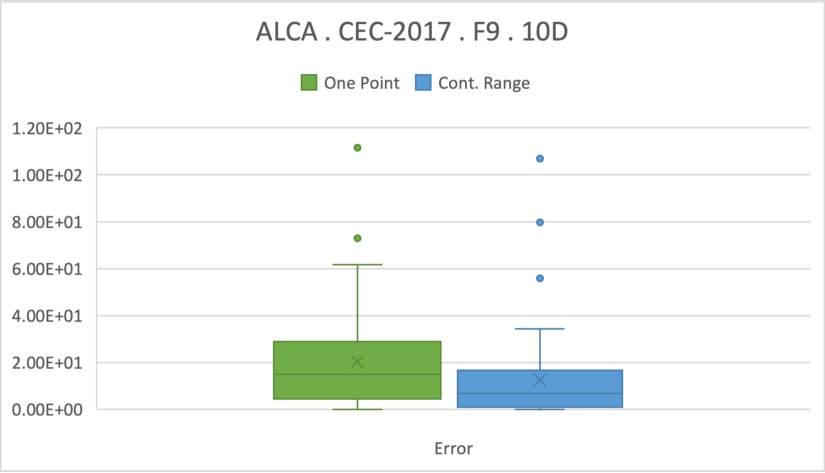
\includegraphics[width=1\linewidth]{img/fig_experiment_F9x10D.pdf} 
        \end{minipage}
        \hfill
        \vspace{0.05 cm}
        \begin{minipage}[h]{0.49\linewidth}
            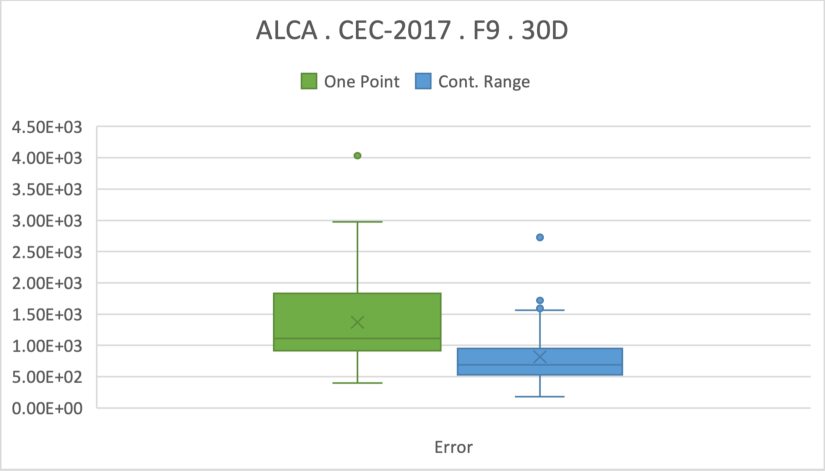
\includegraphics[width=1\linewidth]{img/fig_experiment_F9x30D.pdf} 
        \end{minipage}
        \vfill
        \vspace{0.05 cm}
        \begin{minipage}[h]{0.49\linewidth}
            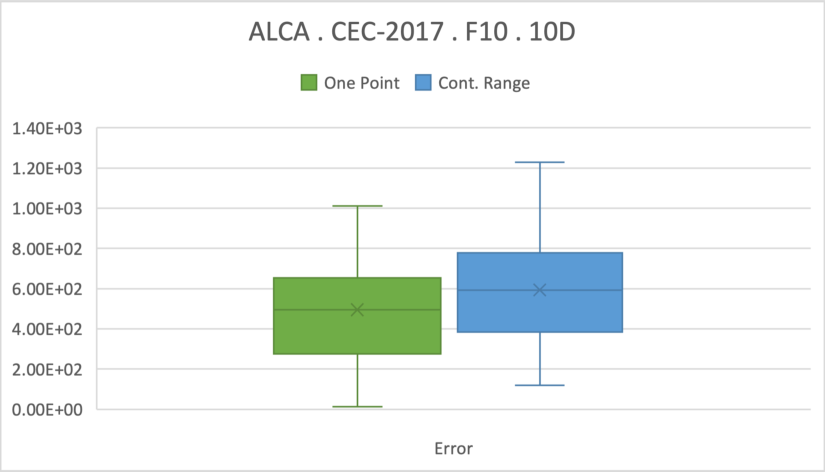
\includegraphics[width=1\linewidth]{img/fig_experiment_F10x10D.pdf} 
        \end{minipage}
        \hfill
        \begin{minipage}[h]{0.49\linewidth}
            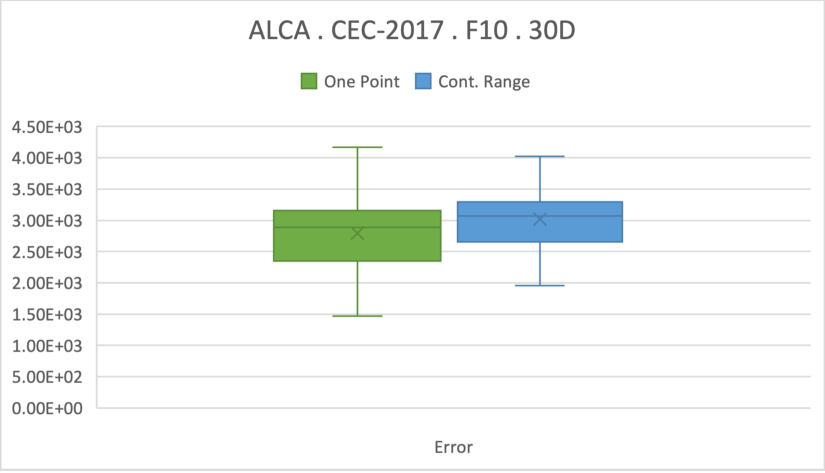
\includegraphics[width=1\linewidth]{img/fig_experiment_F10x30D.pdf} 
        \end{minipage}
        \vfill
        \vspace{0.05 cm}
        \begin{minipage}[h]{0.49\linewidth}
            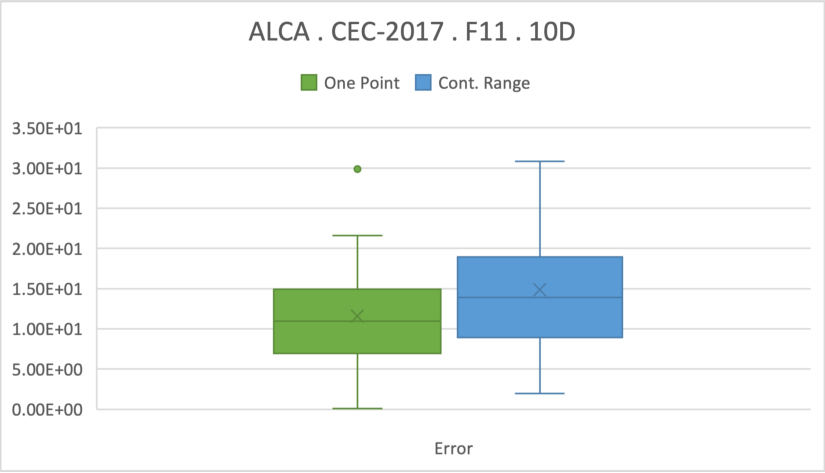
\includegraphics[width=1\linewidth]{img/fig_experiment_F11x10D.pdf} 
        \end{minipage}
        \hfill
        \begin{minipage}[h]{0.49\linewidth}
            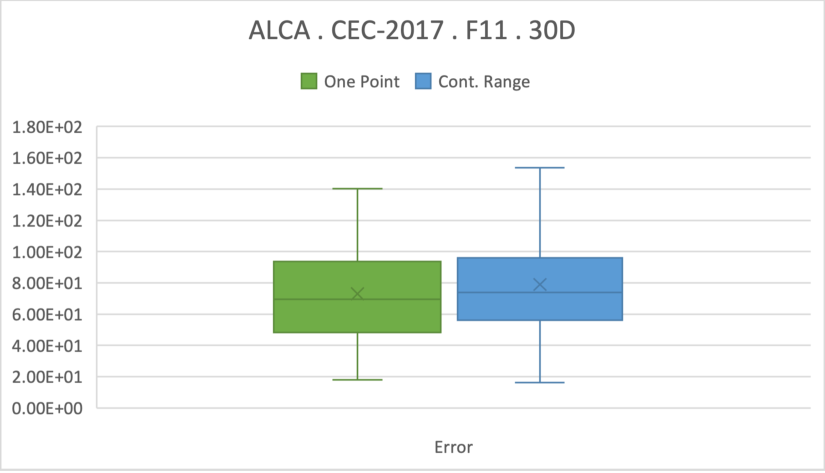
\includegraphics[width=1\linewidth]{img/fig_experiment_F11x30D.pdf} 
        \end{minipage}
        \vfill
        \vspace{0.05 cm}
        \begin{minipage}[h]{0.49\linewidth}
            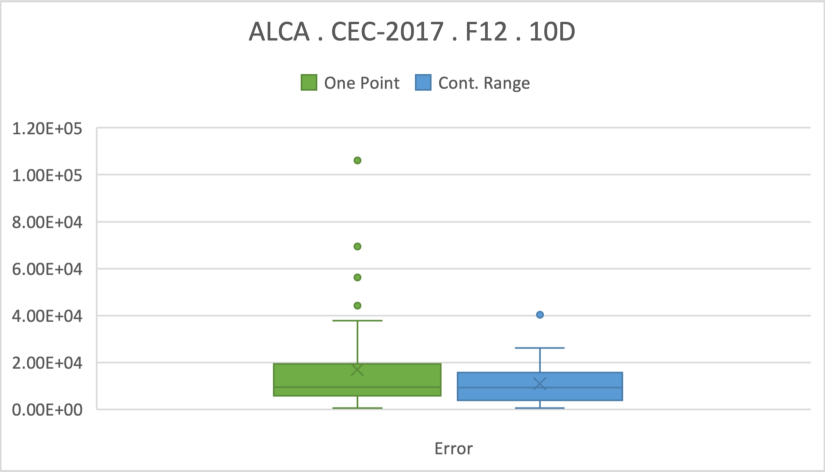
\includegraphics[width=1\linewidth]{img/fig_experiment_F12x10D.pdf} 
        \end{minipage}
        \hfill
        \begin{minipage}[h]{0.49\linewidth}
            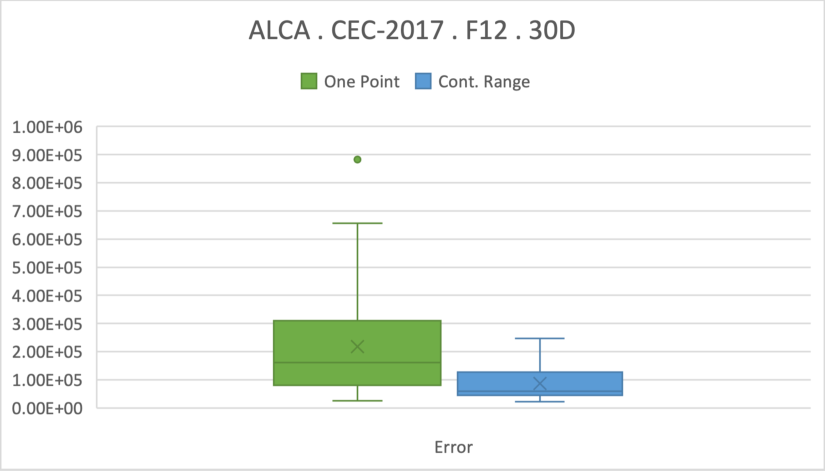
\includegraphics[width=1\linewidth]{img/fig_experiment_F12x30D.pdf} 
        \end{minipage}
        \vfill
        \vspace{0.05 cm}
        \begin{minipage}[h]{0.49\linewidth}
            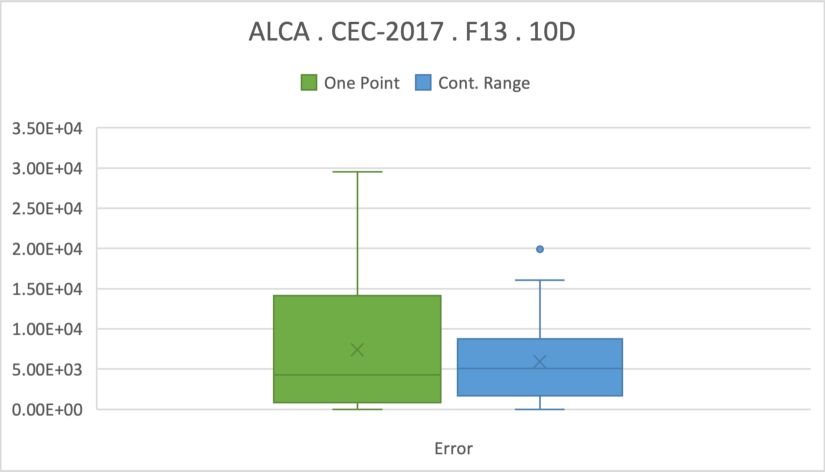
\includegraphics[width=1\linewidth]{img/fig_experiment_F13x10D.pdf} 
        \end{minipage}
        \hfill
        \begin{minipage}[h]{0.49\linewidth}
            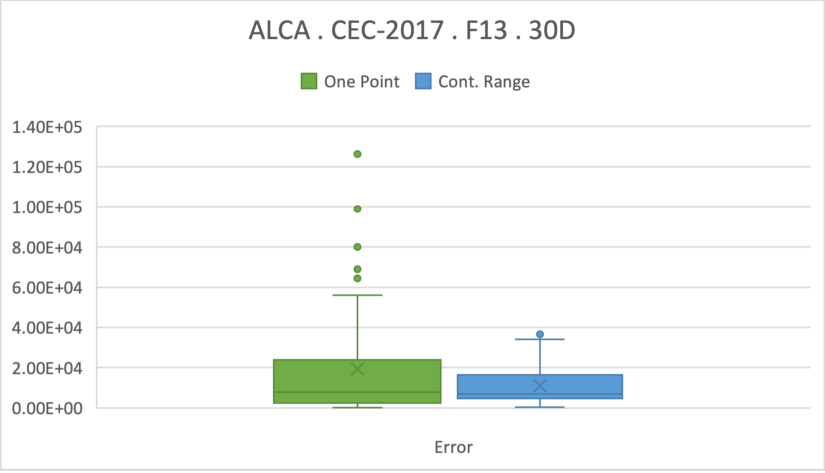
\includegraphics[width=1\linewidth]{img/fig_experiment_F13x30D.pdf} 
        \end{minipage}
        \vfill
        \vspace{0.05 cm}
        \begin{minipage}[h]{0.49\linewidth}
            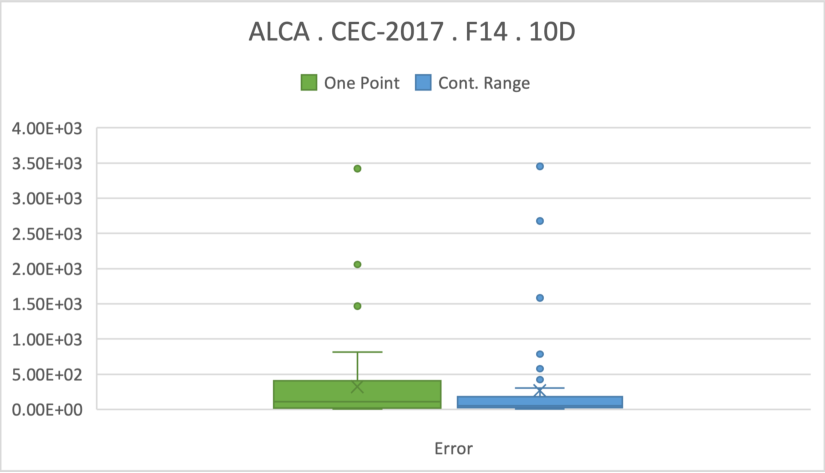
\includegraphics[width=1\linewidth]{img/fig_experiment_F14x10D.pdf} 
        \end{minipage}
        \hfill
        \begin{minipage}[h]{0.49\linewidth}
            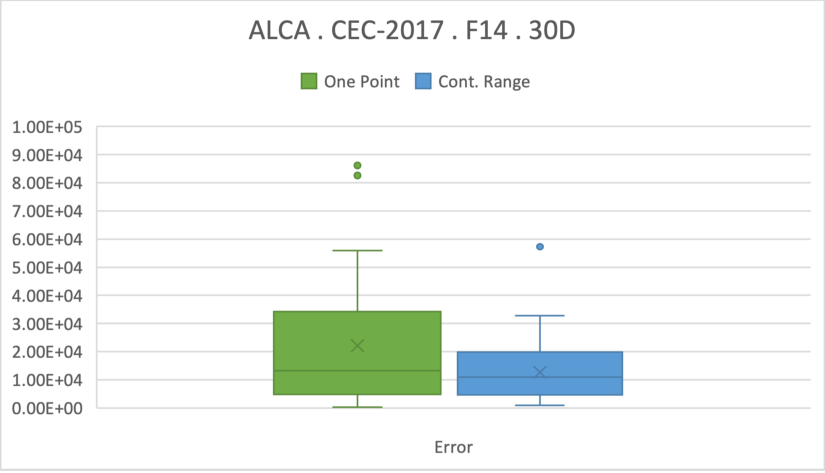
\includegraphics[width=1\linewidth]{img/fig_experiment_F14x30D.pdf} 
        \end{minipage}

        \caption{Box and Whisker charts for mathematical functions F9 to F14. We display the ten and thirty-dimension charts on the left and right sides for the results accumulated in 51 runs.} \label{fig.experiment_F9-F14}
    \end{figure}

    \FloatBarrier

    \begin{figure}[!ht]
        \begin{minipage}[h]{0.49\linewidth}
            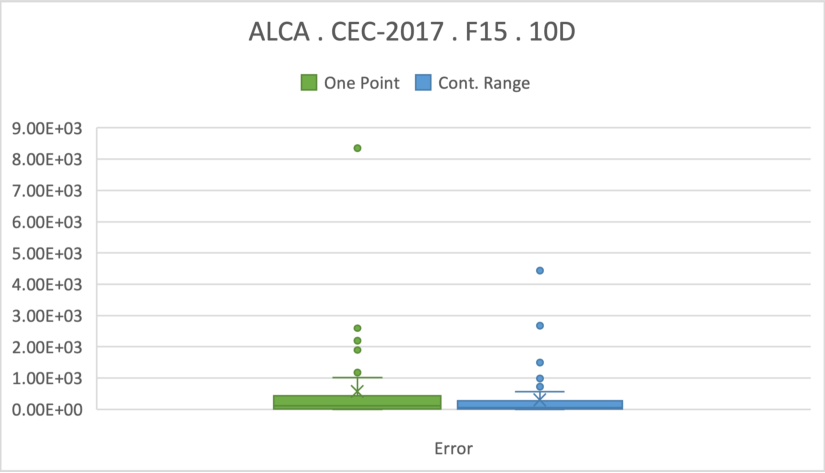
\includegraphics[width=1\linewidth]{img/fig_experiment_F15x10D.pdf} 
        \end{minipage}
        \hfill
        \vspace{0.05 cm}
        \begin{minipage}[h]{0.49\linewidth}
            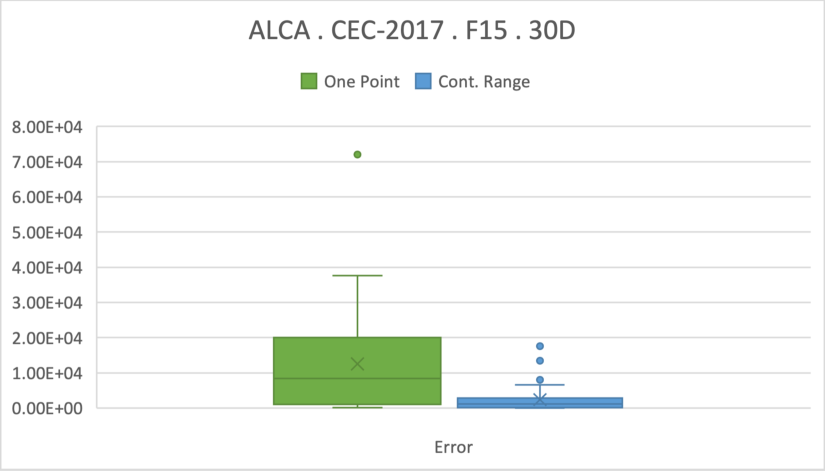
\includegraphics[width=1\linewidth]{img/fig_experiment_F15x30D.pdf} 
        \end{minipage}
        \vfill
        \vspace{0.05 cm}
        \begin{minipage}[h]{0.49\linewidth}
            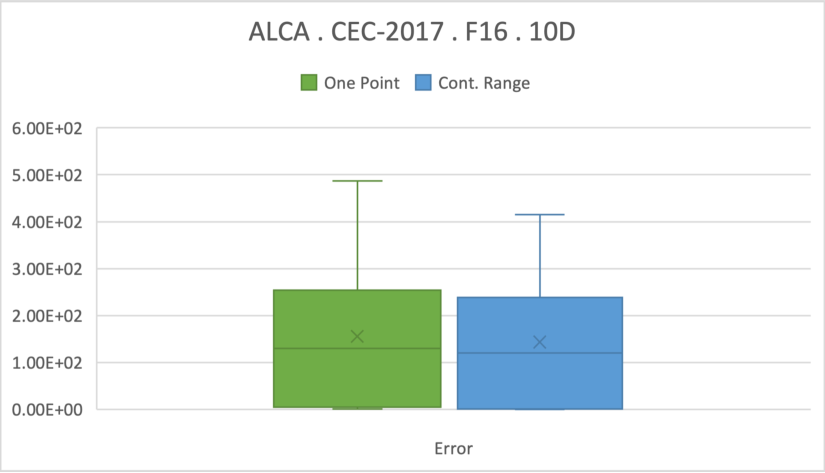
\includegraphics[width=1\linewidth]{img/fig_experiment_F16x10D.pdf} 
        \end{minipage}
        \hfill
        \begin{minipage}[h]{0.49\linewidth}
            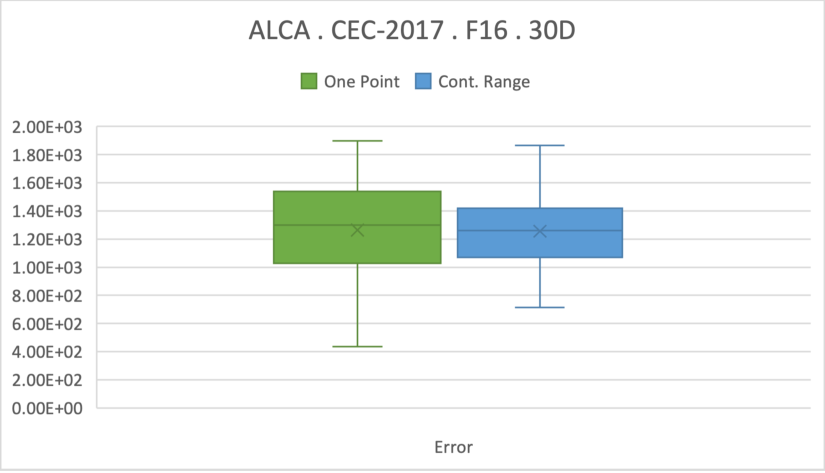
\includegraphics[width=1\linewidth]{img/fig_experiment_F16x30D.pdf} 
        \end{minipage}
        \vfill
        \vspace{0.05 cm}
        \begin{minipage}[h]{0.49\linewidth}
            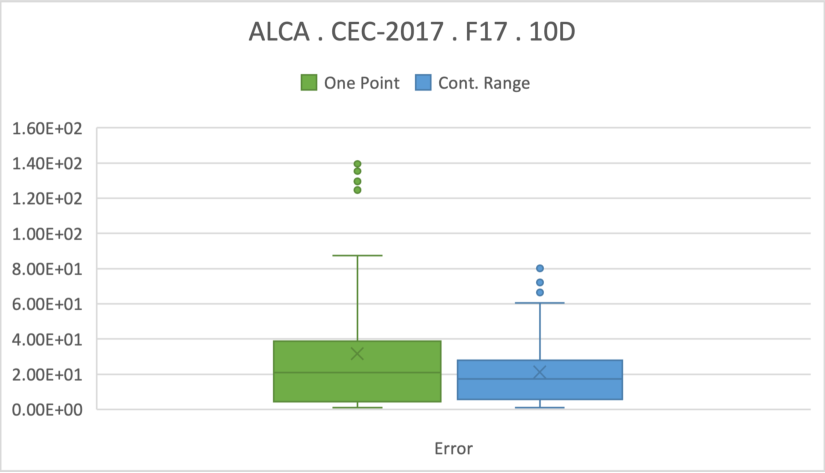
\includegraphics[width=1\linewidth]{img/fig_experiment_F17x10D.pdf} 
        \end{minipage}
        \hfill
        \begin{minipage}[h]{0.49\linewidth}
            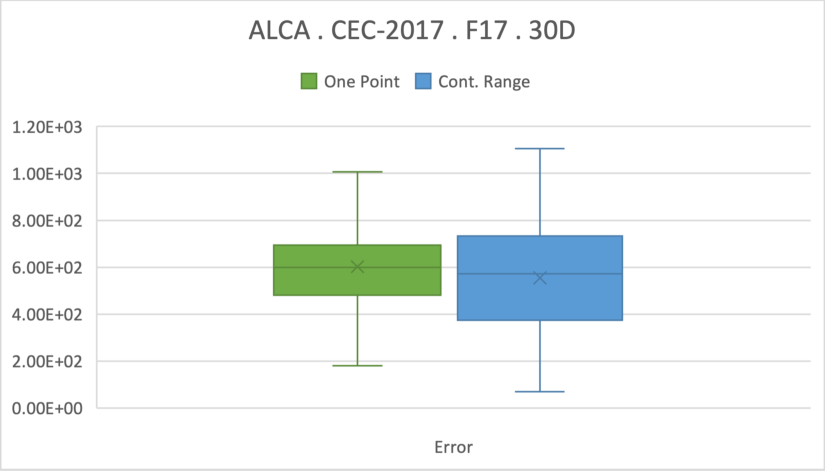
\includegraphics[width=1\linewidth]{img/fig_experiment_F17x30D.pdf} 
        \end{minipage}
        \vfill
        \vspace{0.05 cm}
        \begin{minipage}[h]{0.49\linewidth}
            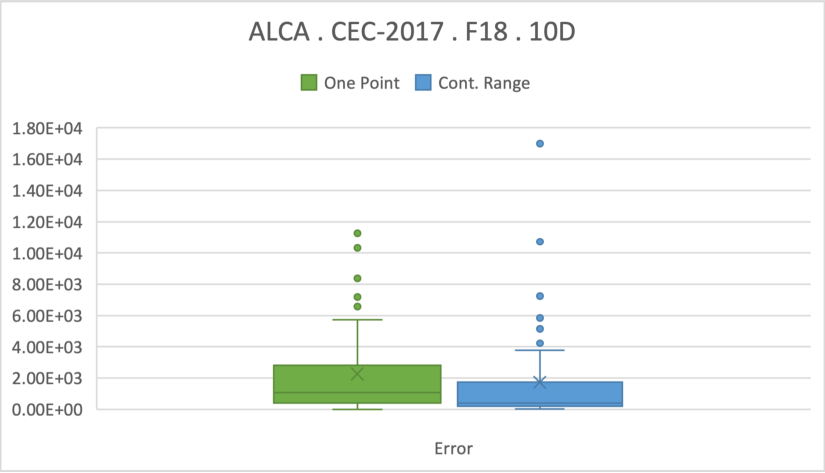
\includegraphics[width=1\linewidth]{img/fig_experiment_F18x10D.pdf} 
        \end{minipage}
        \hfill
        \begin{minipage}[h]{0.49\linewidth}
            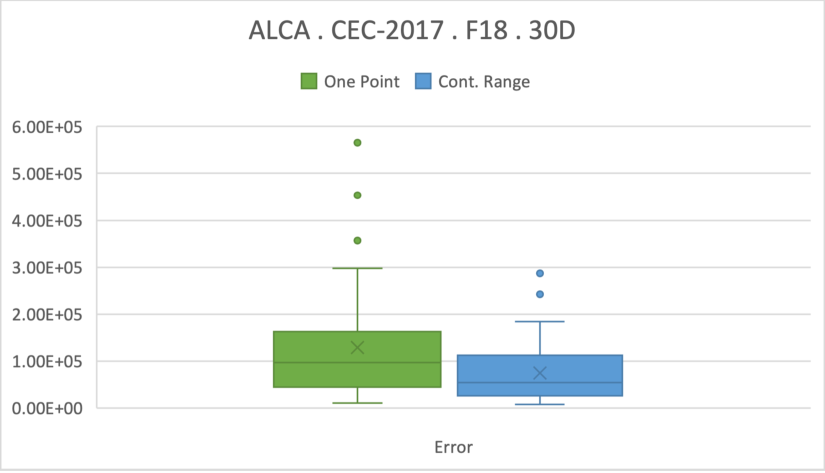
\includegraphics[width=1\linewidth]{img/fig_experiment_F18x30D.pdf} 
        \end{minipage}
        \vfill
        \vspace{0.05 cm}
        \begin{minipage}[h]{0.49\linewidth}
            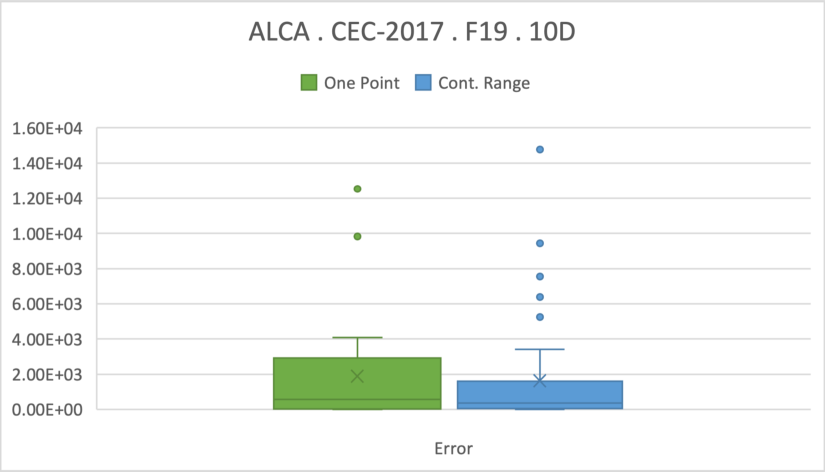
\includegraphics[width=1\linewidth]{img/fig_experiment_F19x10D.pdf} 
        \end{minipage}
        \hfill
        \begin{minipage}[h]{0.49\linewidth}
            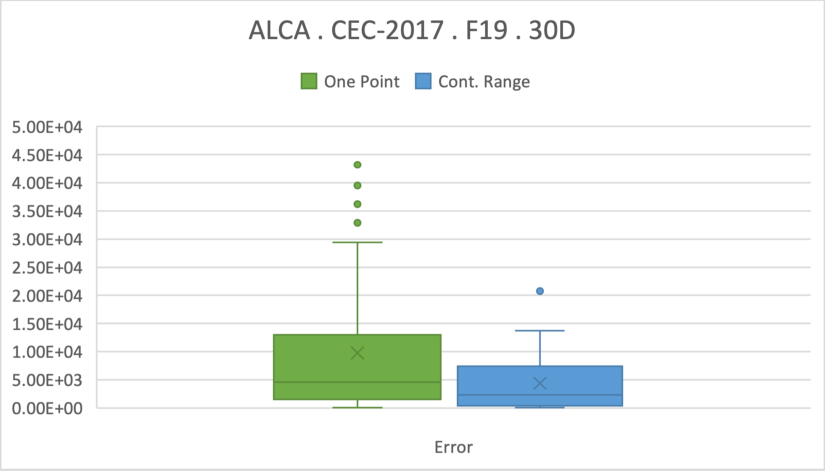
\includegraphics[width=1\linewidth]{img/fig_experiment_F19x30D.pdf} 
        \end{minipage}
        \vfill
        \vspace{0.05 cm}
        \begin{minipage}[h]{0.49\linewidth}
            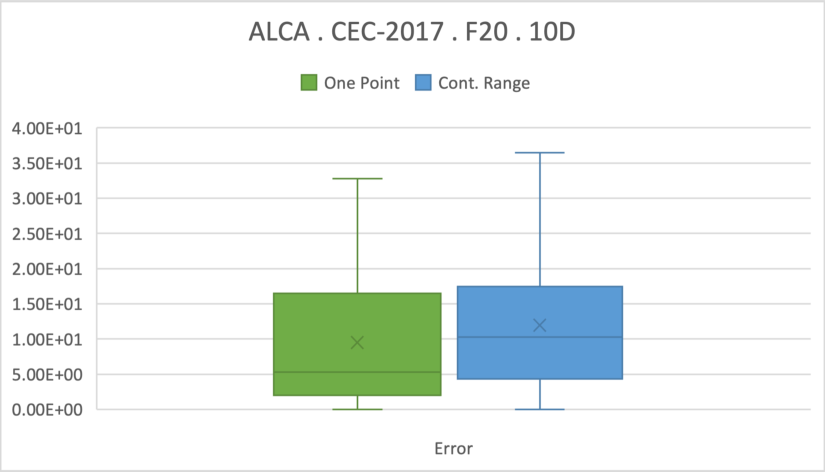
\includegraphics[width=1\linewidth]{img/fig_experiment_F20x10D.pdf} 
        \end{minipage}
        \hfill
        \begin{minipage}[h]{0.49\linewidth}
            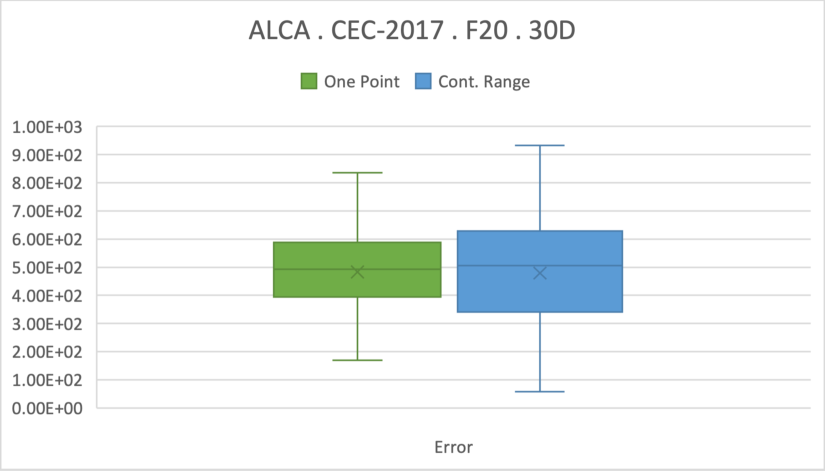
\includegraphics[width=1\linewidth]{img/fig_experiment_F20x30D.pdf} 
        \end{minipage}

        \caption{Box and Whisker charts for mathematical functions F15 to F20. We display the ten and thirty-dimension charts on the left and right sides for the results accumulated in 51 runs.} \label{fig.experiment_F15-F20}
    \end{figure}

    \FloatBarrier

    \begin{figure}[!ht]
        \begin{minipage}[h]{0.49\linewidth}
            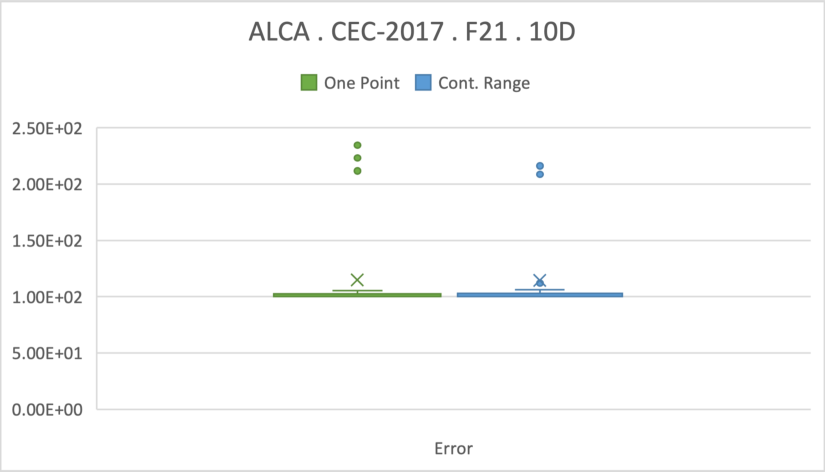
\includegraphics[width=1\linewidth]{img/fig_experiment_F21x10D.pdf} 
        \end{minipage}
        \hfill
        \vspace{0.05 cm}
        \begin{minipage}[h]{0.49\linewidth}
            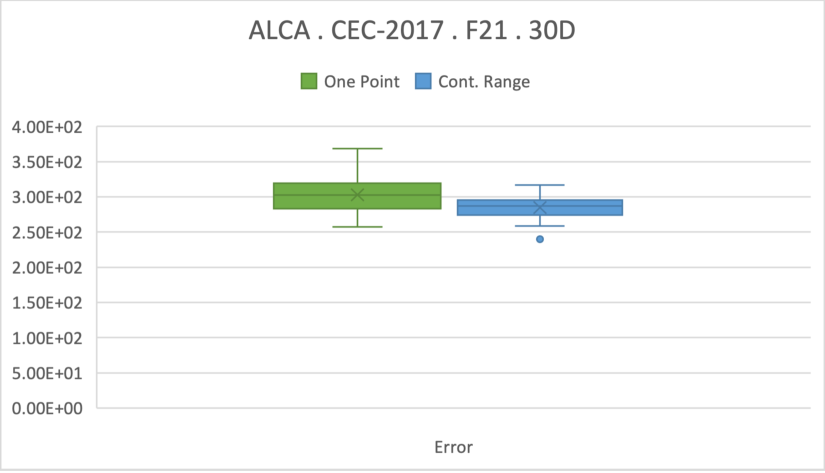
\includegraphics[width=1\linewidth]{img/fig_experiment_F21x30D.pdf} 
        \end{minipage}
        \vfill
        \vspace{0.05 cm}
        \begin{minipage}[h]{0.49\linewidth}
            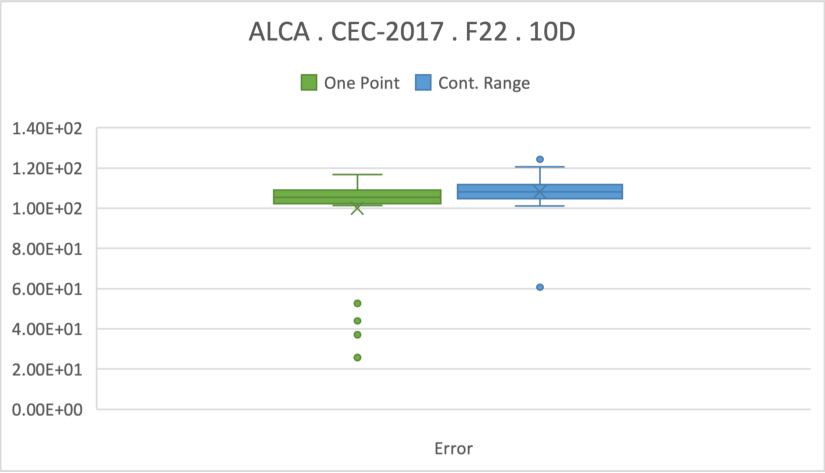
\includegraphics[width=1\linewidth]{img/fig_experiment_F22x10D.pdf} 
        \end{minipage}
        \hfill
        \begin{minipage}[h]{0.49\linewidth}
            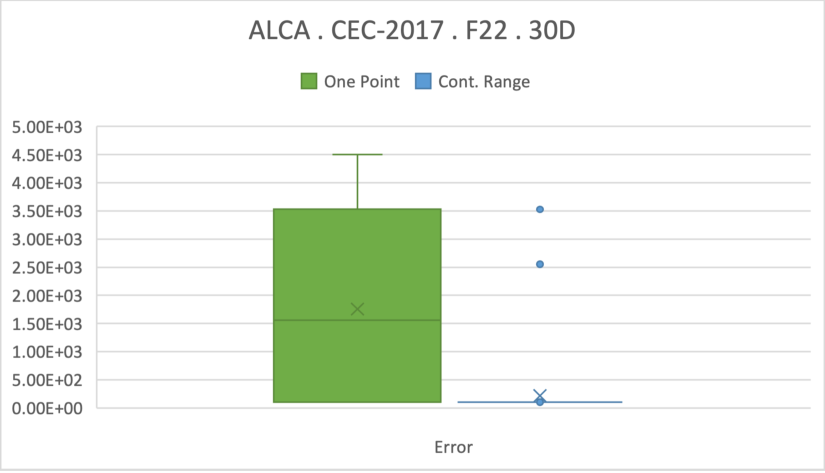
\includegraphics[width=1\linewidth]{img/fig_experiment_F22x30D.pdf} 
        \end{minipage}
        \vfill
        \vspace{0.05 cm}
        \begin{minipage}[h]{0.49\linewidth}
            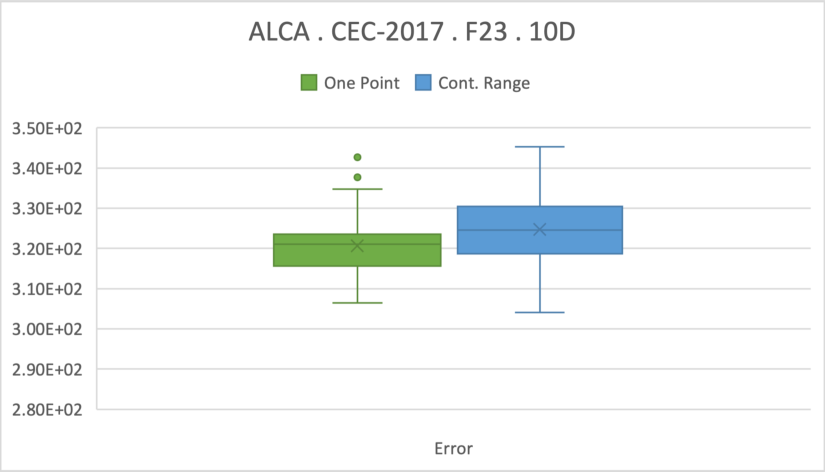
\includegraphics[width=1\linewidth]{img/fig_experiment_F23x10D.pdf} 
        \end{minipage}
        \hfill
        \begin{minipage}[h]{0.49\linewidth}
            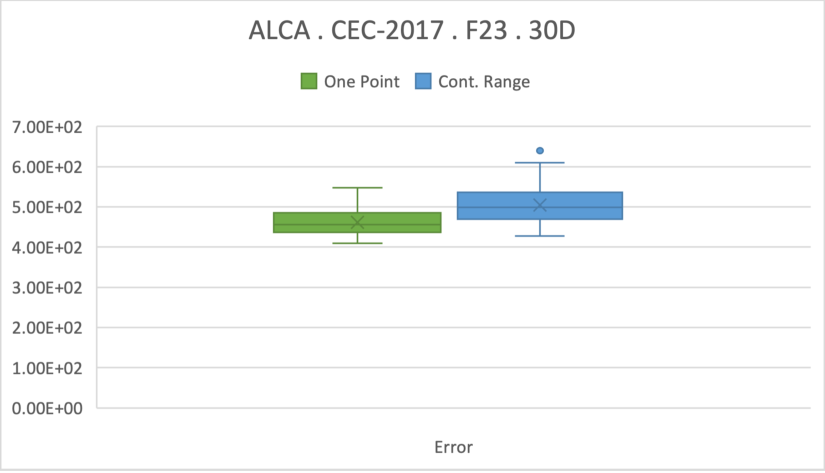
\includegraphics[width=1\linewidth]{img/fig_experiment_F23x30D.pdf} 
        \end{minipage}
        \vfill
        \vspace{0.05 cm}
        \begin{minipage}[h]{0.49\linewidth}
            \includegraphics[width=1\linewidth]{img/fig_experiment_F24x10D.pdf} 
        \end{minipage}
        \hfill
        \begin{minipage}[h]{0.49\linewidth}
            \includegraphics[width=1\linewidth]{img/fig_experiment_F24x30D.pdf} 
        \end{minipage}
        \vfill
        \vspace{0.05 cm}
        \begin{minipage}[h]{0.49\linewidth}
            \includegraphics[width=1\linewidth]{img/fig_experiment_F25x10D.pdf} 
        \end{minipage}
        \hfill
        \begin{minipage}[h]{0.49\linewidth}
            \includegraphics[width=1\linewidth]{img/fig_experiment_F25x30D.pdf} 
        \end{minipage}
        \vfill
        \vspace{0.05 cm}
        \begin{minipage}[h]{0.49\linewidth}
            \includegraphics[width=1\linewidth]{img/fig_experiment_F26x10D.pdf} 
        \end{minipage}
        \hfill
        \begin{minipage}[h]{0.49\linewidth}
            \includegraphics[width=1\linewidth]{img/fig_experiment_F26x30D.pdf} 
        \end{minipage}

        \caption{Box and Whisker charts for mathematical functions F21 to F26. We display the ten and thirty-dimension charts on the left and right sides for the results accumulated in 51 runs.} \label{fig.experiment_F21-F26}
    \end{figure}

    \FloatBarrier

    \begin{figure}[!ht]
        \begin{minipage}[h]{0.49\linewidth}
            \includegraphics[width=1\linewidth]{img/fig_experiment_F27x10D.pdf} 
        \end{minipage}
        \hfill
        \vspace{0.05 cm}
        \begin{minipage}[h]{0.49\linewidth}
            \includegraphics[width=1\linewidth]{img/fig_experiment_F27x30D.pdf} 
        \end{minipage}
        \vfill
        \vspace{0.05 cm}
        \begin{minipage}[h]{0.49\linewidth}
            \includegraphics[width=1\linewidth]{img/fig_experiment_F28x10D.pdf} 
        \end{minipage}
        \hfill
        \begin{minipage}[h]{0.49\linewidth}
            \includegraphics[width=1\linewidth]{img/fig_experiment_F28x30D.pdf} 
        \end{minipage}
        \vfill
        \vspace{0.05 cm}
        \begin{minipage}[h]{0.49\linewidth}
            \includegraphics[width=1\linewidth]{img/fig_experiment_F29x10D.pdf} 
        \end{minipage}
        \hfill
        \begin{minipage}[h]{0.49\linewidth}
            \includegraphics[width=1\linewidth]{img/fig_experiment_F29x30D.pdf} 
        \end{minipage}
        \vfill
        \vspace{0.05 cm}
        \begin{minipage}[h]{0.49\linewidth}
            \includegraphics[width=1\linewidth]{img/fig_experiment_F30x10D.pdf} 
        \end{minipage}
        \hfill
        \begin{minipage}[h]{0.49\linewidth}
            \includegraphics[width=1\linewidth]{img/fig_experiment_F30x30D.pdf} 
        \end{minipage}

        \caption{Box and Whisker charts for mathematical functions F27 to F30. We display the ten and thirty-dimension charts on the left and right sides for the results accumulated in 51 runs.} \label{fig.experiment_F27-F30}
    \end{figure}

    \FloatBarrier


\section{Discussion}
    \label{section.discussion}

    For our experimentation, we executed fifty-one independent runs per specified dimension for each CEC-2017 mathematical benchmark function. We registered the following values: best-found error average and standard deviation to calculate the statistical Z-Test value. We summarized our results in the following tables, with the labels described next:

    \begin{itemize}
        \item   Fx:          is the mathematical benchmark function.
        \item   Mean:        is the average of the best-found error.
        \item   St-Dev:      is the computed error standard deviation. 
        \item   Z:           is the calculated statistical Z-Test value.
    \end{itemize}

    To find and determine the best alternative, finalized with a statistical Z-Test with a ninety-five percent confidence level. Here are the results' statistics values: Table~\ref{tab.condensed_evaluation_10D} shows the condensed ALCA evaluation results for the CEC-2017 functions running on ten dimensions (D) for alternatives One Point and Continuous Range crossover; Table~\ref{tab.condensed_evaluation_30D} displays the condensed ALCA evaluation results for the CEC-2017 mathematical operations running on thirty D for the same crossover alternatives.

    \begin{table}[]
    \scriptsize
    \centering
    \caption{Condensed ALCA evaluation results for the CEC-2017 functions running on ten dimensions for alternatives One Point and Continuous Range crossover.}\label{tab.condensed_evaluation_10D}
    \begin{tabular}{@{}lllllllll@{}}
    \toprule
    \multicolumn{9}{c}{\textbf{ALCA . CEC-2017 . 10D}} \\ \midrule
    Crossover &  & \multicolumn{3}{c}{One Point Xover} &  & \multicolumn{3}{c}{Cont. Range Xover} \\
    Fx &  & Mean & Std. Dev. & Z &  & Mean & Std. Dev. & Z \\
    F1 &  & 2.14E+03 & 2.14E+03 & 5.42E+00 &  & 4.43E+02 & 6.46E+02 & \textbf{-5.42E+00} \\
    F2 &  & 1.81E-03 & 2.63E-03 & 2.38E+00 &  & 8.54E-04 & 1.16E-03 & \textbf{-2.38E+00} \\
    F3 &  & 4.19E-04 & 1.16E-03 & 2.49E+00 &  & 1.33E-05 & 2.20E-05 & \textbf{-2.49E+00} \\
    F4 &  & 6.00E+00 & 1.31E+01 & 2.00E+00 &  & 2.31E+00 & 1.78E+00 & \textbf{-2.00E+00} \\
    F5 &  & 1.53E+01 & 7.06E+00 & 2.45E+00 &  & 1.24E+01 & 4.14E+00 & \textbf{-2.45E+00} \\
    F6 &  & 6.05E-04 & 9.22E-04 & -1.43E+00 &  & 2.53E-03 & 9.61E-03 & 1.43E+00 \\
    F7 &  & 3.15E+01 & 9.06E+00 & 2.26E+00 &  & 2.76E+01 & 8.38E+00 & \textbf{-2.26E+00} \\
    F8 &  & 1.78E+01 & 7.38E+00 & 8.00E+00 &  & 8.62E+00 & 3.53E+00 & \textbf{-8.00E+00} \\
    F9 &  & 2.02E+01 & 2.24E+01 & 1.85E+00 &  & 1.25E+01 & 1.96E+01 & \textbf{-1.85E+00} \\
    F10 &  & 4.96E+02 & 2.26E+02 & \textbf{-2.02E+00} &  & 5.94E+02 & 2.63E+02 & 2.02E+00 \\
    F11 &  & 1.16E+01 & 6.01E+00 & \textbf{-2.44E+00} &  & 1.49E+01 & 7.48E+00 & 2.44E+00 \\
    F12 &  & 1.70E+04 & 1.99E+04 & 2.00E+00 &  & 1.10E+04 & 8.21E+03 & \textbf{-2.00E+00} \\
    F13 &  & 7.39E+03 & 8.16E+03 & 1.08E+00 &  & 5.94E+03 & 5.03E+03 & -1.08E+00 \\
    F14 &  & 3.24E+02 & 6.05E+02 & 4.65E-01 &  & 2.67E+02 & 6.34E+02 & -4.65E-01 \\
    F15 &  & 5.70E+02 & 1.31E+03 & 1.25E+00 &  & 3.07E+02 & 7.46E+02 & -1.25E+00 \\
    F16 &  & 1.56E+02 & 1.28E+02 & 5.05E-01 &  & 1.43E+02 & 1.18E+02 & -5.05E-01 \\
    F17 &  & 3.17E+01 & 3.65E+01 & 1.81E+00 &  & 2.11E+01 & 1.98E+01 & \textbf{-1.81E+00} \\
    F18 &  & 2.26E+03 & 2.88E+03 & 9.03E-01 &  & 1.73E+03 & 3.06E+03 & -9.03E-01 \\
    F19 &  & 1.88E+03 & 3.24E+03 & 4.11E-01 &  & 1.63E+03 & 2.95E+03 & -4.11E-01 \\
    F20 &  & 9.50E+00 & 8.32E+00 & -1.35E+00 &  & 1.20E+01 & 9.92E+00 & 1.35E+00 \\
    F21 &  & 1.15E+02 & 3.86E+01 & 4.93E-02 &  & 1.15E+02 & 3.58E+01 & -4.93E-02 \\
    F22 &  & 1.00E+02 & 2.07E+01 & \textbf{-2.57E+00} &  & 1.08E+02 & 8.70E+00 & 2.57E+00 \\
    F23 &  & 3.21E+02 & 7.31E+00 & \textbf{-2.53E+00} &  & 3.25E+02 & 8.91E+00 & 2.53E+00 \\
    F24 &  & 3.28E+02 & 8.06E+01 & 5.36E+00 &  & 2.15E+02 & 1.28E+02 & \textbf{-5.36E+00} \\
    F25 &  & 4.35E+02 & 2.61E+01 & 1.39E+00 &  & 4.28E+02 & 2.41E+01 & -1.39E+00 \\
    F26 &  & 3.99E+02 & 1.25E+02 & 7.55E-01 &  & 3.82E+02 & 9.35E+01 & -7.55E-01 \\
    F27 &  & 3.88E+02 & 1.03E+01 & -5.43E-01 &  & 3.90E+02 & 1.13E+01 & 5.43E-01 \\
    F28 &  & 4.11E+02 & 7.92E+01 & 1.93E+00 &  & 3.80E+02 & 8.46E+01 & \textbf{-1.93E+00} \\
    F29 &  & 3.00E+02 & 4.32E+01 & 7.44E-01 &  & 2.94E+02 & 3.30E+01 & -7.44E-01 \\
    F30 &  & 3.21E+02 & 1.52E+02 & -7.14E-01 &  & 3.44E+02 & 1.81E+02 & 7.14E-01 \\
    \textbf{Total (W)} &  & \multicolumn{2}{c}{\textbf{One Point Xover}} & \multicolumn{1}{c}{\textbf{4 of 30}} &  & \multicolumn{2}{c}{\textbf{Cont. Range Xover}} & \multicolumn{1}{c}{\textbf{12 of 30}} \\ \bottomrule
    \end{tabular}
    \end{table}

    \FloatBarrier

    We performed the statistical Z-Test for both crossover alternatives with a 95 percent confidence level. When the One Point passes the test, the Z value is highlighted in bold on the left column. When the Continuous Range passes the statistical test, the Z value is highlighted in bold on the right column. Where we did not find enough evidence to declare one choice as the best alternative, no value was highlighted.

    \begin{table}[]
    \scriptsize
    \centering
    \caption{Condensed ALCA evaluation results for the CEC-2017 functions running on thirty dimensions for alternatives One Point and Continuous Range crossover.}\label{tab.condensed_evaluation_30D}    
    \begin{tabular}{@{}lllllllll@{}}
    \toprule
    \multicolumn{9}{c}{\textbf{ALCA . CEC-2017 . 30D}} \\ \midrule
    Crossover &  & \multicolumn{3}{c}{One Point Xover} &  & \multicolumn{3}{c}{Cont. Range Xover} \\
    Fx &  & Mean & Std. Dev. & Z &  & Mean & Std. Dev. & Z \\
    F1 &  & 4.92E+03 & 6.21E+03 & 1.60E+00 &  & 3.35E+03 & 3.33E+03 & -1.60E+00 \\
    F2 &  & 9.21E+06 & 4.77E+07 & 1.37E+00 &  & 6.96E+04 & 2.50E+05 & -1.37E+00 \\
    F3 &  & 1.17E+02 & 1.18E+02 & 4.33E+00 &  & 4.16E+01 & 3.85E+01 & \textbf{-4.33E+00} \\
    F4 &  & 7.17E+01 & 3.14E+01 & -5.29E-01 &  & 7.46E+01 & 2.52E+01 & 5.29E-01 \\
    F5 &  & 9.38E+01 & 2.41E+01 & 4.61E-01 &  & 9.18E+01 & 2.04E+01 & -4.61E-01 \\
    F6 &  & 4.67E-03 & 1.02E-02 & \textbf{-2.42E+00} &  & 2.28E-02 & 5.26E-02 & 2.42E+00 \\
    F7 &  & 1.55E+02 & 3.04E+01 & -3.88E-01 &  & 1.58E+02 & 3.44E+01 & 3.88E-01 \\
    F8 &  & 9.94E+01 & 2.43E+01 & 6.82E+00 &  & 7.29E+01 & 1.32E+01 & \textbf{-6.82E+00} \\
    F9 &  & 1.37E+03 & 7.21E+02 & 4.60E+00 &  & 8.19E+02 & 4.64E+02 & \textbf{-4.60E+00} \\
    F10 &  & 2.79E+03 & 5.59E+02 & \textbf{-2.22E+00} &  & 3.02E+03 & 4.63E+02 & 2.22E+00 \\
    F11 &  & 7.31E+01 & 2.72E+01 & -1.09E+00 &  & 7.90E+01 & 2.75E+01 & 1.09E+00 \\
    F12 &  & 2.18E+05 & 1.94E+05 & 4.61E+00 &  & 8.73E+04 & 5.95E+04 & \textbf{-4.61E+00} \\
    F13 &  & 1.95E+04 & 2.73E+04 & 2.09E+00 &  & 1.10E+04 & 8.96E+03 & \textbf{-2.09E+00} \\
    F14 &  & 2.22E+04 & 2.14E+04 & 2.83E+00 &  & 1.27E+04 & 1.06E+04 & \textbf{-2.83E+00} \\
    F15 &  & 1.25E+04 & 1.41E+04 & 4.96E+00 &  & 2.37E+03 & 3.82E+03 & \textbf{-4.96E+00} \\
    F16 &  & 1.26E+03 & 3.45E+02 & 1.49E-01 &  & 1.26E+03 & 2.49E+02 & -1.49E-01 \\
    F17 &  & 6.02E+02 & 1.76E+02 & 1.17E+00 &  & 5.54E+02 & 2.36E+02 & -1.17E+00 \\
    F18 &  & 1.29E+05 & 1.17E+05 & 2.92E+00 &  & 7.44E+04 & 6.27E+04 & \textbf{-2.92E+00} \\
    F19 &  & 9.78E+03 & 1.16E+04 & 3.04E+00 &  & 4.38E+03 & 5.08E+03 & \textbf{-3.04E+00} \\
    F20 &  & 4.83E+02 & 1.69E+02 & 1.02E-01 &  & 4.79E+02 & 2.03E+02 & -1.02E-01 \\
    F21 &  & 3.03E+02 & 2.44E+01 & 4.40E+00 &  & 2.85E+02 & 1.62E+01 & \textbf{-4.40E+00} \\
    F22 &  & 1.76E+03 & 1.72E+03 & 6.07E+00 &  & 2.16E+02 & 5.84E+02 & \textbf{-6.07E+00} \\
    F23 &  & 4.62E+02 & 3.06E+01 & \textbf{-5.27E+00} &  & 5.05E+02 & 4.97E+01 & 5.27E+00 \\
    F24 &  & 6.45E+02 & 7.43E+01 & \textbf{-2.31E+00} &  & 6.78E+02 & 7.03E+01 & 2.31E+00 \\
    F25 &  & 3.85E+02 & 1.49E+01 & \textbf{-3.06E+00} &  & 3.97E+02 & 2.40E+01 & 3.06E+00 \\
    F26 &  & 2.40E+03 & 4.88E+02 & -1.23E+00 &  & 2.61E+03 & 1.17E+03 & 1.23E+00 \\
    F27 &  & 4.94E+02 & 1.23E+01 & 2.98E-01 &  & 4.93E+02 & 1.95E+01 & -2.98E-01 \\
    F28 &  & 4.63E+02 & 4.29E+01 & 9.26E+00 &  & 3.98E+02 & 2.58E+01 & \textbf{-9.26E+00} \\
    F29 &  & 9.22E+02 & 2.36E+02 & 1.55E+00 &  & 8.56E+02 & 2.00E+02 & -1.55E+00 \\
    F30 &  & 3.53E+03 & 4.15E+03 & 4.09E+00 &  & 1.08E+03 & 1.04E+03 & \textbf{-4.09E+00} \\
    \multicolumn{1}{c}{\textbf{Total (W)}} & \multicolumn{1}{c}{\textbf{}} & \multicolumn{2}{c}{\textbf{One Point Xover}} & \multicolumn{1}{c}{\textbf{5 of 30}} & \multicolumn{1}{c}{\textbf{}} & \multicolumn{2}{c}{\textbf{Cont. Range Xover}} & \multicolumn{1}{c}{\textbf{13 of 30}} \\ \bottomrule
    \end{tabular}
    \end{table}

    \FloatBarrier

\section{Conclusions}
    \label{section.conclusions}

    To validate our research, we performed the statistical Z-Test with a ninety-five percent confidence level to analyze the alternatives we present in this proposal. In the ten-dimension category, we found that One Point crossover was the better alternative on four occasions, while our Continuous Range proposal was better on twelve other functions out of thirty. For the thirty-dimensions category, the One Point crossover was better on five occasions, while the Continuous Range crossover was the best alternative on another thirteen. Our experiment results confirm that our solution can be considered an adequate alternative.

    Some researchers might consider our proposal similar to what is used by algorithms such as Differential Evolution, where we consider our proposal to be a variation of existing proposals because we expect this new operator to allow the offspring to continue exploring new search spaces with the birth of individuals. Experimental results indicate that our proposed operator may be a viable alternative for the canonical One Point crossover.

    Based on the analysis of our results, we have shown that the proposed crossover alternative for the reproduction of individuals in a population obtains good results. Therefore, it can be valuable in other evolutionary algorithms where the information of individuals has a structure similar to that of the genetic code. However, with some adaptation, it could be helpful in different types of algorithms, such as Particle Swarm Optimization. In future work, we could investigate a combination between the canonical One Point Crossover strategy and randomly alternating with the proposed Continuous Range Crossover.


\begin{acknowledgement}
    This paper has been supported in part by TecNM Project 18186.23-P.
\end{acknowledgement}

% ---- Bibliography ----
% BibTeX users should specify bibliography style 'splncs04'.
% References will then be sorted and formatted in the correct style.
%

\bibliographystyle{splncs03_unsrt}
%\bibliographystyle{splncs04}
\bibliography{bib/bibliografia.bib}

\end{document}

% TO-DO: Turnitin.
